\section{Técnicas de simulación a distintas escalas}

Dentro de la física, la química y las ciencias de los materiales existen diversas
técnicas computacionales para desarrollar modelos capaces de predecir y entender 
las propiedades de algún sistema en particular. Estos modelos no son más que 
abstracciones matemáticas o lógicas de la realidad que permiten obtener dicha 
información de interés a costa de renunciar a otra \cite{franco2013}. 
En la Figura \ref{fig:escalas} se muestran aplicaciones específicas de 
simulaciones numéricas que cubren distintos intervalos de escalas espaciales y 
temporales. Con respecto a las baterías de litio, se han estudiado distintas
componentes de las mismas con técnicas tales como DFT \cite{he2019}, Dinámica 
molecular \cite{yao2022}, Monte Carlo \cite{mercer2017}, Monte Carlo cinético 
\cite{gavilan2021}, Dinámica mesoescala \cite{ryan2019} y Modelos del continuo
\cite{brosa2022}. En particular, en esta tesis se utilizan las técnicas 
resaltadas con colores en la Figura \ref{fig:escalas} para estudiar distintos 
aspectos de materiales de interés en el área de las baterías de ion-litio.

\begin{figure}[h!]
    \centering
    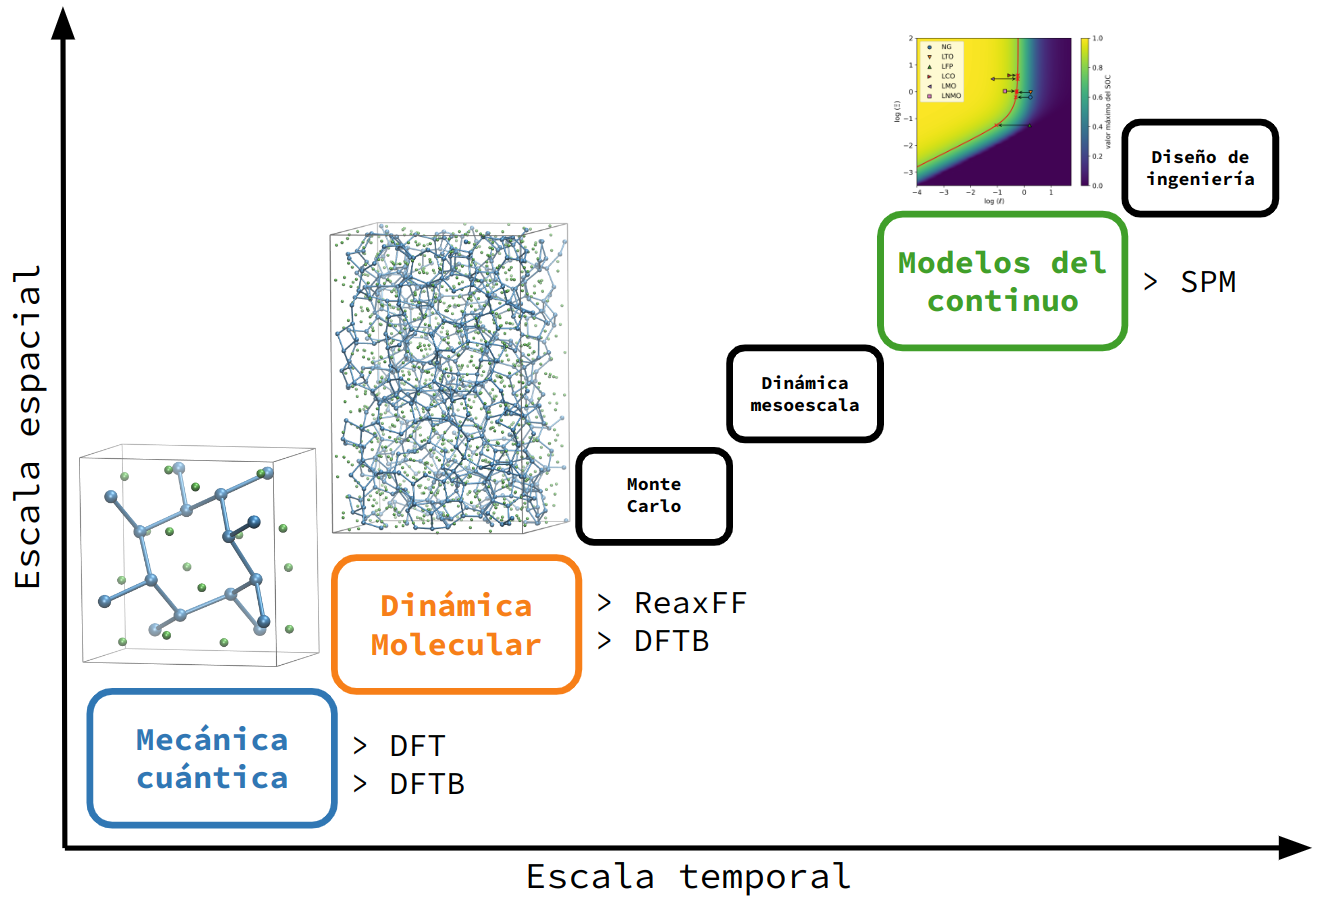
\includegraphics[width=.8\textwidth]{Metodos/tecnicas/escalas.png}
    \caption{Esquema de escalas espaciales y temporales relativas de distintas 
    técnicas de simulaciones computacionales. Se destacan con colores aquellas que 
    se utilizaron en esta tesis mientras que se mencionan otras.}
    \label{fig:escalas}
\end{figure}

Los métodos tradicionales de prueba y error requieren demasiado tiempo como 
para seguir el ritmo rápido de crecimiento en la demanda de sistemas de 
almacenamiento y transporte de energía, que actualmente se encuentran limitados por los
materiales disponibles. Esto ha atraído la atención de investigadores e ingenieros 
hacia el desarrollo de modelos computacionales, desde la escala atómica hasta la 
escala del continuo, y la integración de las mismas, para tener una herramienta 
predictiva para resolver los problemas relacionados a los electrones, los átomos, 
los clusters, las partículas, los electrodos, las celdas e incluso el pack de 
baterías \cite{shi2016}. En particular, en la escala atómica usualmente se tienen
predicciones bajo equilibrio termodinámico de propiedades como la estructura, 
transformaciones de fase, energías de activación, entre otras, como se lo realiza
en la Parte \ref{p:silicio} de esta tesis para el caso de los ánodos de silicio. 
Además de esto, se busca encontrar relaciones que mapeen dichas propiedades con 
descriptores más simples de obtener \cite{juan2021}, como se propone en la Parte
\ref{p:fast-charging} de esta tesis al ajustar datos experimentales con un modelo
del continuo.
